\section{Specyfikacja sprzętu}

\subsection{Schemat architektury}

\begin{figure}[H]
	\centering
	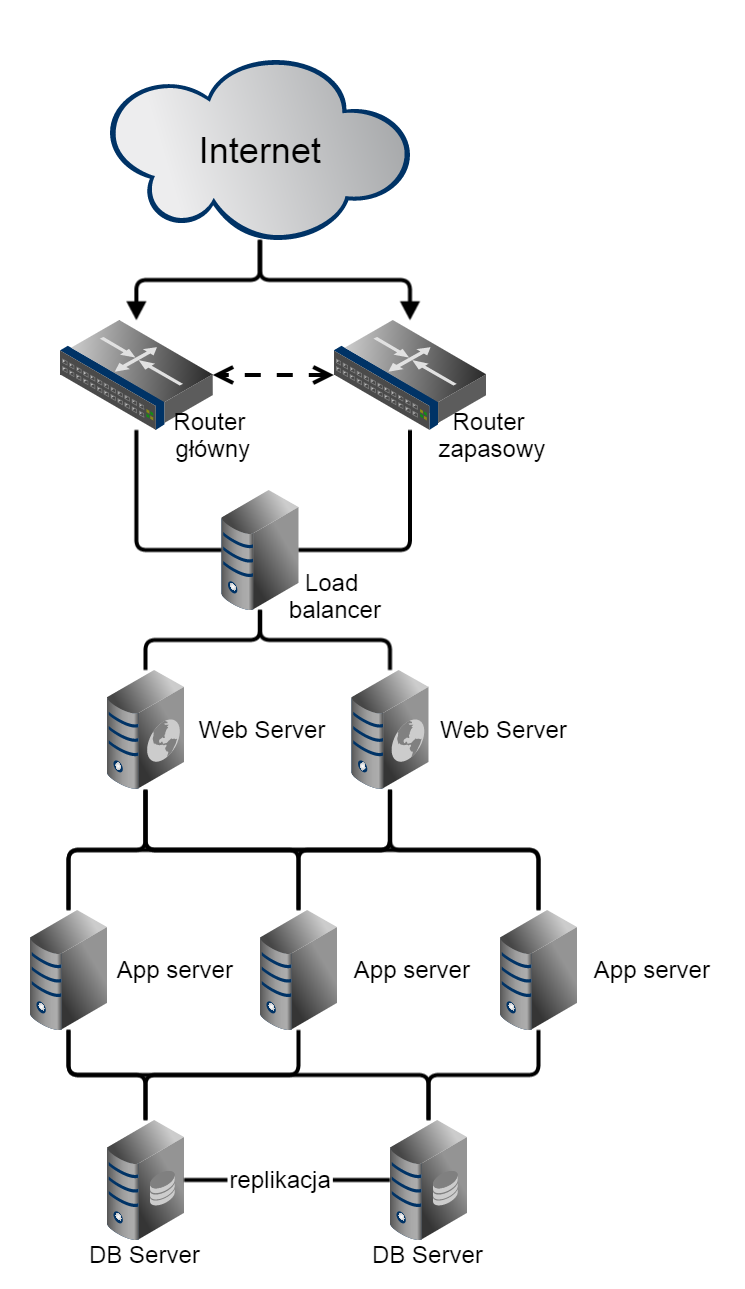
\includegraphics[height=0.8\textheight]{img/architektura}
	\caption{Schemat architektury \label{fig:labelArchitecture}}
\end{figure}


Jak uwidoczniono na \ref*{fig:labelArchitecture} na wejściu żądania będą obsługiwany przez router główny, któremu towarzyszył będzie router zapasowy w przypadku, kiedy router główny nie będzie w stanie obsłużyć żądania. Następnie wybierany będzie Web Server, który będzie obsługiwał zgłoszenie (w zależności od poziomu obciążenia serwerów, decydować o tym będzie Load Balancer). W analogiczny sposób wybierany będzie serwer aplikacyjny, pośredniczący w obsłudze.

W odniesieniu do serwerów bazy danych zastosowany będzie mechanizm replikacji danych, który ma zagwarantować bezpieczeństwo przechowywanych informacji (ochronę przed ich utratą w wyniku awarii jednego z serwerów).

\subsection{Oszacowanie rozmiarów systemu}

W chwili obecnej firma posiada w ewidencji:

\begin{itemize}
\item[--] około 50 pojazdów
\item[--] około 800 telefonów
\item[--] około 1500 komputerów stacjonarnych
\item[--] około 2500 monitorów komputerowych
\item[--] około 2000 laptopów
\item[--] około 100 serwerów
\item[--] około 200 sztuk sprzętu serwerowego
\item[--] około 10000 sztuk innego drobnego sprzętu komputerowego
\item[--] około 300 nośników z oprogramowaniem
\item[--] około 200 licencji na użytkowanie oprogramowania (jedna licencja na wiele stanowisk)
\end{itemize}

Oznacza to, że w ewidencji firmy jest ponad 17 tysięcy przedmiotów i
licencji na oprogramowanie. Ponieważ firma się intensywnie rozwija
należy założyć, że system będzie obsługiwał co najmniej 30 tysięcy
przedmiotów. W chwili obecnej firma zatrudnia około 1500
pracowników. Ponieważ firma przeżywa intensywny rozwój konieczne jest
zwymiarowanie systemu na poziomie co najmniej dwu krotności obecnego
zatrudnienia to jest 3000 pracowników. System należy do grupy systemów
wspierających funkcjonowanie przedsiębiorstwa i nie będzie
wykorzystywany w ramach podstawowych zadania pracowników. Należy zatem
założyć, że nie wszyscy pracownicy będą go używali w tym samym
czasie. W związku z tym należy założyć, że równocześnie system będzie
używany przez około 10\% pracowników czyli 300 osób. Powyższe szacunki
są zgodne z wymaganiami niefunkcjonalnymi przedstawionymi w
\ref{wymagania_niefunkcjonalne}.

\subsection{Rozkład obciążenia na poszczególne warstwy}

Aplikacja w architekturze trójwarstwowej posiada budowę bardzo
modularną, przez co możliwe jest rozmieszczenie różnych elementów na
odpowiednich maszynach. Dzięki takiemu rozmieszczeniu każda z warstw
może być wykonywana na sprzęcie dostosowanym do jej zadań. Ponieważ
każda warstwa wykonuje inne zadania to znacząco też różni się
charakterystyka sprzętu, który należy wykorzystać w danej warstwie.

\subsubsection{Warstwa prezentacji}

Warstwa prezentacji odpowiedzialna jest za wyświetlanie użytkownikowi
treści. Implementacja tej warstwy zostanie wykonana z użyciem języka
JavaScript wraz z technologiami HTML oraz CSS. Ponadto dodatkowa
funkcjonalność zostanie zaimplementowana przy użyciu biblioteki
jQuerry. Pomimo, iż zarówno serwer jak i klienci znajdować się będą w
sieci wewnętrznej przedsiębiorstwa należy zapewnić odpowiedni poziom
bezpieczeństwa poprzez wykorzystanie protokołu SSL/TLS.

Z perspektywy wymaganych zasobów sprzętowych wymagania dla tej warstwy
można podzielić na dwie części. Pierwsza z nich dotyczy wymagań co do
urządzenia na którym treść będzie prezentowana. Konieczne jest aby
takie urządzenie wyposażone było w przeglądarkę obsługującą
JavaScript. Druga część z wymagań sprzętowych dotyczy serwera www, do
którego kierowane będą żądania. Od tego urządzenia wymaga się przede
wszystkim wysokiej wydajności, krótkiego czasu odpowiedzi oraz
możliwości obsługi wielu klientów jednocześnie. Istotne jest również
zapewnienie wysokiej dostępności tego serwera.

\subsubsection{Warstwa logiki biznesowej}

Warstwa logiki biznesowej odpowiedzialna jest za przetwarzanie żądań
klienta w sposób zgodny z prawami rządzącymi organizacją. Zostanie ona
zaimplementowana w technologii J2EE. Jako serwer aplikacyjny wybrano
JBoos Application Server.

Z perspektywy wymaganych zasobów warstwa ta posiada analogiczne
wymagania jak warstwa prezentacji. Oznacza to, że istotna dostępność,
krótki czas odpowiedzi oraz możliwość obsługi wielu klientów
równocześnie. Te abstrakcyjne wymagania tej warstwy na sprzęt
przekładają się na duże zapotrzebowanie na procesor (w tym ich
liczbę), rozmiar pamięci RAM oraz szybkość odpowiedzi dysku twardego,
natomiast już sam rozmiar tego dysku może być nie zbyt duży.

\subsubsection{Warstwa danych}

Warstwa danych odpowiedzialna jest za przetwarzanie i przechowywanie
danych w sposób zapewniający ich spójność oraz trwałość. W tej
warstwie zostanie wykorzystana technologia Oracle DataBase 12c w
wersji Enterprise Edition. Jest to najnowsza wersja bazy danych od
Oracle i posiada wiele zaawansowanych mechanizmów, wpływających na
wydajność jak i bezpieczeństwo przechowywanych danych.

Z perspektywy wymaganych zasobów sprzętowych warstwa ta posiada
analogiczne wymagania co poprzednia lecz są one tutaj bardziej
krytyczne, gdyż zbyt długie przetwarzanie zapytania przez bazę danych
znacząco wydłuża czas odpowiedzi aplikacji. Należy również pamiętać o
dostosowaniu rozmiaru pamięci operacyjnej oraz zamontowaniu
odpowiedniej liczby wydajnych dysków twardych wraz z zapewnieniem ich
replikacji w celu zabezpieczenia się przed utrata danych.

\subsection{Sprzęt}

Budowa nowego systemu zarządzania przedmiotami i licencjami wymaga
znacznej rozbudowy dotychczasowej infrastruktury IT firmy.

\subsubsection{Warstwa prezentacji oraz aplikacji}

Część kliencka budowanego systemu będzie uruchamiana poprzez
przeglądarkę na komputerach pracowników firmy. Dzięki temu część
warstwy prezentacji, którą należy umieścić na serwerze składa się
wyłącznie z serwera WWW. Aby zatem ograniczyć konieczne zasoby
sprzętowe, a także opóźnienia w komunikacji pomiędzy warstwą
prezentacji, a warstwą aplikacji zdecydowano umieścić je na wspólnej
maszynie. Ponieważ klient ma wysokie wymagania co do dostępności
systemu, należy zakupić dwa serwery, które będą współdziałały i
dzieliły obciążenie pomiędzy siebie, a w razie awarii jednego z nich
drugi będzie w stanie zapewnić pełną funkcjonalność.


Jako serwer www oraz aplikacyjny powinna zostać wykorzystana maszyna,
która posiada wysoko wydajne procesory oraz pamięć RAM. Ważna jest
również możliwość montażu dysków twardych o krótkim czasie dostępu. W
związku z powyższym zdecydowano o wykorzystaniu serwerów Dell
PowerEdge R630.

\begin{figure}[H]
	\centering
	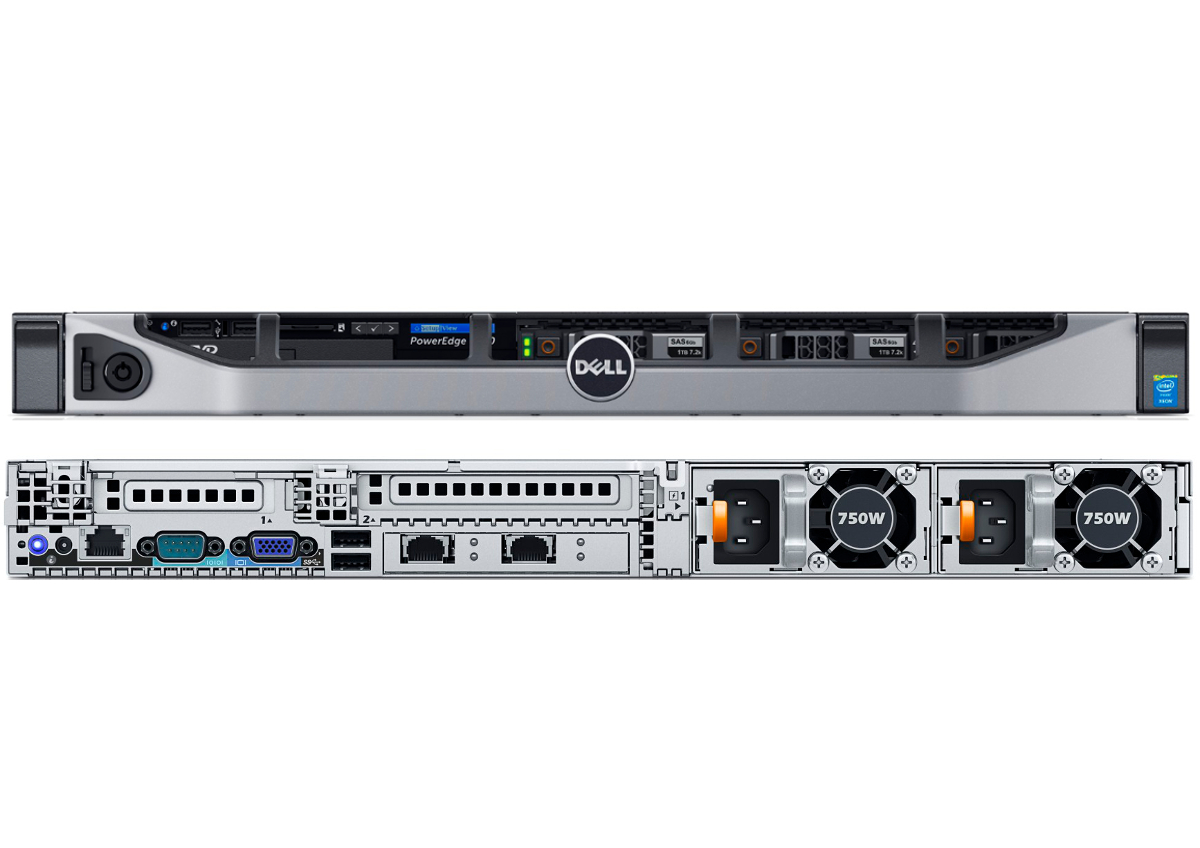
\includegraphics[width=\textwidth]{img/r630.jpg}
	\caption{Dell PowerEdge R630}
\end{figure}

Jest to wysoko wydajny serwer, który dzięki małych rozmiarów oszczędzi
miejsce w serwerowni oraz cechuje się niskim zużyciem
energii. Parametry techniczne serwera:

\begin{description}
\item[procesor] 2 sockety procesora (dla Intel® Xeon® E5 2600 v3)
\item[chipset] Intel C610
\item[pamięć RAM] do 768 GB (24 sloty DIMM) DDR4
\item[pamięć trwała] do 10 dysków (1,8 TB każdy)
\item[kontroler RAID] PERC H730P
\item[złącza I/O] do 3 złącz PCIe
\item[karta sieciowa] 4 x 1Gb, 2 x 1Gb + 2 x 10Gb, 4 x 10Gb
\item[obudowa] Rack 1U
\item[zasilanie] 2x 750W HotPlug
\end{description}

Aby serwer spełnił stawiane przed nim wymagania wydajnościowe należy
zakupić go w następującej konfiguracji:

\begin{description}
\item[procesor] 2x Intel® Xeon® Processor E5-2697 v3
\item[chipset] Intel C610
\item[pamięć RAM] 8x 16 GB DDR4
\item[pamięć trwała] 8x 146 GB 15k SAS (RAID 10)
\item[kontroler RAID] PERC H730P
\item[złącza I/O] do 3 złącz PCIe
\item[karta sieciowa] 4 x 1Gb, 2 x 1Gb + 2 x 10Gb, 4 x 10Gb
\item[obudowa] Rack 1U
\item[zasilanie] 2x 750W HotPlug
\end{description}

Zastosowanie dwóch serwerów o wskazanych parametrów pozwoli sprostać
wszystkim wymaganiom stawianym przez klienta. Ponadto zapewniona jest
możliwość skalowania dostarczonego rozwiązania poprzez dodanie
kolejnego serwera aplikacji lub rozbudowę (głównie pamięć operacyjna)
posiadanych już serwerów.

\subsubsection{Warstwa danych}

Serwer bazy danych powinien pozwalać na gromadzenie znacznej ilości
danych. Konieczne jest również zapewnienie redundantnego drugiego
serwera bazy danych, aby równoważyć obciążenie oraz zapewnić wysoką
dostępność. W celu zapewnienie odpowiednich możliwości w zakresie
przechowywania i przetwarzania dużej ilości danych postanowiono
wykożystać dwa serwery Dell PowerEdge R920.

\begin{figure}[H]
	\centering
	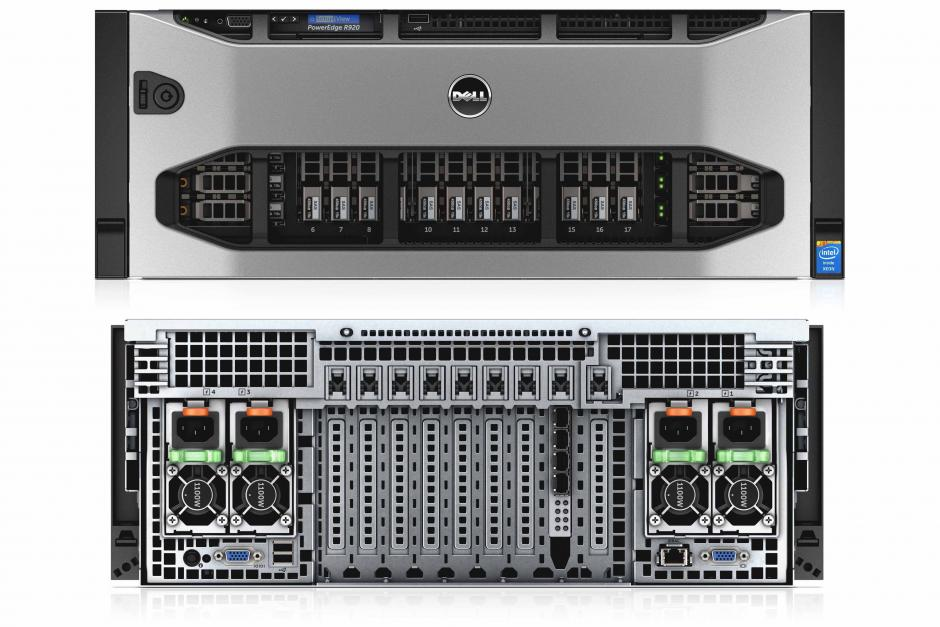
\includegraphics[width=\textwidth]{img/r920.jpg}
	\caption{Dell PowerEdge R920}
\end{figure}

Jest to wysokiej klasy serwer, którego parametry pozwolą na
przetwarzanie danych w czasie rzeczywistym. Parametry techniczne
serwera:

\begin{description}
\item[procesor] 4 sockety procesora (dla Intel Xeon E7-4800 v2 lub E7-8800 v2)
\item[chipset] Intel C602J
\item[pamięć RAM] do 6TB (96 slotów DIMM) DDR3L, RDIMM, LR-DIMM
\item[pamięć trwała] do 24 dysków (1,2 TB każdy)
\item[kontroler RAID] PERC H730P
\item[złącza I/O] do 10 złącz PCIe
\item[karta sieciowa] Intel Ethernet X540 10Gb BT DP + I350 1Gb BT DP
\item[karta graficzna] Matrox® G200 with 8MB memory
\item[obudowa] Rack 4U
\item[zasilanie] 4x 1100W HotPlug
\end{description}

Maksymalne parametry techniczne wybranego serwera znacząco
przewyższają bieżące zapotrzebowanie firmy dlatego wykorzystana
będzie następująca konfiguracja:

\begin{description}
\item[procesor] 2x Intel® Xeon® Processor E7-8880 v2 (37.5M Cache, 2.50 GHz)
\item[chipset] Intel C602J
\item[pamięć RAM] 8x 16 GB
\item[pamięć trwała] 2x 146 GB 15k SAS + 8x 1.2 TB
\item[kontroler RAID] PERC H730P
\item[złącza I/O] do 10 złącz PCIe
\item[karta sieciowa] Intel Ethernet X540 10Gb BT DP + I350 1Gb BT DP
\item[karta graficzna] Matrox® G200 with 8MB memory
\item[obudowa] Rack 4U
\item[zasilanie] 4x 1100W HotPlug
\end{description}

Zastosowana konfiguracja jest zdecydowanie wystarczająca dla
bieżących wymagań firmy, a zastosowanie wysokiej klasy serwera
pozostawia duże możliwości w zakresie skalowalności, dzięki czemu
serwery te będzie można dostosować do potrzeb intensywnie rozwijającej
się firmy. Dzięki wsparciu technologii wirtualizacji sprzętowej serwer
ten będzie mógł być efektywnie współdzielony z pozostałymi modułami
budowanego systemu.

